\documentclass{article}
\usepackage[utf8]{inputenc}
\usepackage{graphicx}

\title{CIS 678 Project 1}
\author{Thomas Bailey}
\date{January 2019}



% Default fixed font does not support bold face
\DeclareFixedFont{\ttb}{T1}{txtt}{bx}{n}{12} % for bold
\DeclareFixedFont{\ttm}{T1}{txtt}{m}{n}{12}  % for normal

% Custom colors
\usepackage{color}
\definecolor{deepblue}{rgb}{0,0,0.5}
\definecolor{deepred}{rgb}{0.6,0,0}
\definecolor{deepgreen}{rgb}{0,0.5,0}

\usepackage{listings}

% Python style for highlighting
\newcommand\pythonstyle{\lstset{
language=Python,
basicstyle=\ttm,
otherkeywords={self},             % Add keywords here
keywordstyle=\ttb\color{deepblue},
emph={MyClass,__init__},          % Custom highlighting
emphstyle=\ttb\color{deepred},    % Custom highlighting style
stringstyle=\color{deepgreen},
frame=tb,                         % Any extra options here
showstringspaces=false            % 
}}


% Python environment
\lstnewenvironment{python}[1][]
{
\pythonstyle
\lstset{#1}
}
{}

% Python for external files
\newcommand\pythonexternal[2][]{{
\pythonstyle
\lstinputlisting[#1]{#2}}}

% Python for inline
\newcommand\pythoninline[1]{{\pythonstyle\lstinline!#1!}}

\begin{document}

\maketitle

\section{Introduction}

For this project I chose to use Python 3, because I am familiar with the language and it was recommended by the professor. My design approach for this project was primarily functional. I separated the necessary tasks into functions and used the functions to achieve the desired result.

\section{Pre-processing}

I wrote a function that read the data file line by line, added each pair as a key value set in a dictionary, and returned the dictionary. If the value was 'nan', I omitted the pair. As a result, my dictionary has fewer than 744 pairs. Because of this, for the purposes of prediction, I treated my data set like it did contain a months worth of hours of data, even though there were fewer; the first hour into the next month would be hour n + 1, where n is the number of data pairs. 

\section{Visualization}

I used matplotlib's pyplot library to plot the scatter for my data. The visualization tells me that the number of downloads had a sharp increase towards the end of the month.

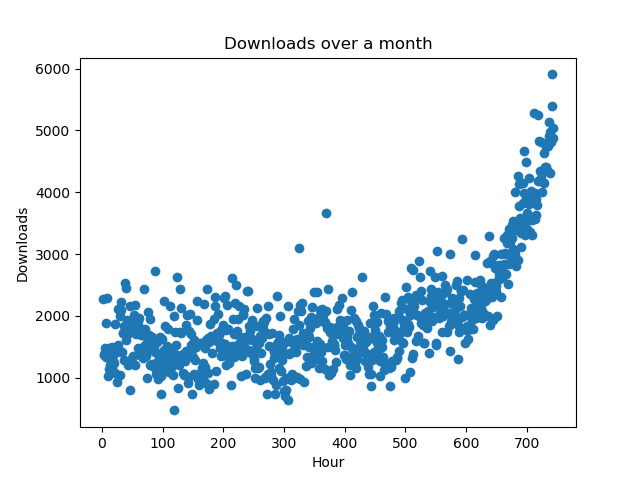
\includegraphics[scale=0.6]{scatter.png}

\section{Analysis}

I used a linear regression to fit a line to my data points. Based on my regression equation, I predicted that we could expect 3257 downloads at noon on the fifth day of the next month. However, I don't think the linear analysis captures the uptick in downloads towards the end of the month.

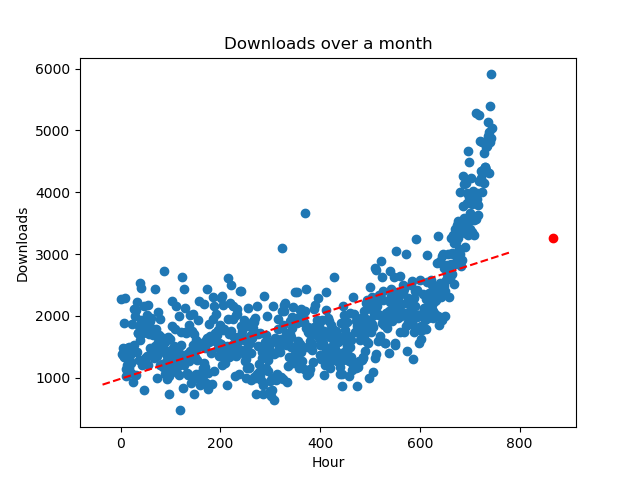
\includegraphics[scale=0.6]{linear_regression_prediction.png}

A polynomial regression might have produced a more accurate prediction. I implemented a function to test out a  polynomial regression with order 6. Using the new regression, I predicted that we could expect around 16158 downloads at noon on the fifth day of the next month.

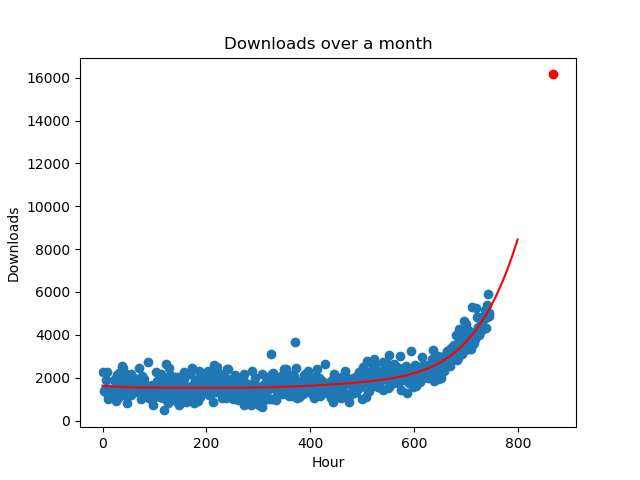
\includegraphics[scale=0.6]{polynomial_regression_deg6.png}

\section{Source Code}

\begin{python}
import matplotlib.pyplot as plt
import numpy as np

def read_data(filename):
    f = open(filename, "r")
    result = {}
    for line in f.readlines():
        hour, purchases = line.strip("\n").split(",")
        if purchases == 'nan': continue
        result[int(hour)] = int(purchases)
    return result

def add_scatter(data):
    plt.clf()
    plt.title('Downloads over a month')
    plt.xlabel('Hour')
    plt.ylabel('Downloads')
    plt.scatter(data.keys(), data.values())
    
def linear_regression(data):
    # Initialize values for slope intercept calculation
    sigx = sum(data.keys())
    sigy = sum(data.values())
    sigxy = sum(x*y for x, y in data.items())
    sigx_2 = sum(x*x for x in data.keys())
    sigy_2 = sum(y*y for y in data.values())
    n = len(data)
    # Calculate slope intercept
    slope = (n*sigxy - sigx*sigy) / (n*sigx_2 - sigx*sigx)
    intercept = (sigy - slope*sigx) / n
    return slope, intercept

def calculate_y_with_coefficients(x, coeffs):
    o = len(coeffs)
    y = 0
    for i in range(o):
        y += coeffs[i]*x**i
    return y

def add_line(slope, intercept):
    axes = plt.gca()
    x_vals = np.array(axes.get_xlim())
    y_vals = intercept + slope * x_vals
    plt.plot(x_vals, y_vals, '--', color='r')

def predict(slope, intercept, x_value):
    return intercept + slope*x_value
    
def show():
    plt.show()

def demo():
    # Read in & clean the data
    data = read_data("downloads.txt")

    # Show scatterplot
    add_scatter(data)
    show()

    # Calculate slope intercept of linear regression
    slope, intercept = linear_regression(data)

    # Predict downloads at noon on the fifth day of the next month
    hour = 12+24*5+len(data)
    download_prediction = predict(slope, intercept, hour)
    print("Linear regression for x {}: {}".format(hour,
                        round(download_prediction)))

    # Show scatterplot with linear regression & predicted download point
    add_scatter(data)
    add_line(slope, intercept)
    plt.plot(hour, download_prediction, 'ro')
    show()

    # Show scatterplot with polynomial regression degree 6
    polynomial_regression(6)

def polynomial_regression(degree):
    data = read_data("downloads.txt")
    coeffs = np.polyfit(list(data.keys()),
            list(data.values()), degree).tolist()[::-1]
    x = list(x for x in range(800))
    y = [calculate_y_with_coefficients(x, coeffs) for x in x]
    add_scatter(data)
    plt.plot(x, y, 'r')

    # Prediction
    hour = 12+24*5+len(data)
    prediction = calculate_y_with_coefficients(hour, coeffs)
    print("Polynomial regression for x {}: {}".format(hour,
                                round(prediction)))
    plt.plot(hour, prediction, 'ro')
    show()

if __name__ == "__main__":
    demo()
\end{python}

\section{Output}

\begin{verbatim}
    
\end{verbatim}

[baileyth@arch05 ml]\$ python main.py

Linear regression prediction for hour 868: 3257

Polynomial regression prediction for hour 868: 16158

[baileyth@arch05 ml]\$

\section{Challenges}

I wasn't able to get a correct polynomial regression implementation without using the numpy built-in method.

\end{document}
